%%%%%%%%%%%%%%%%%%%%%%%%%%%%%%%%%%%%%%%%%%%%%%%%%%%%%%%%%%%%%%%%%%%%%%%%%%%%%%%%%%
\begin{frame}[fragile]\frametitle{}
\begin{center}
{\Large Introduction}
\end{center}
\end{frame}


%%%%%%%%%%%%%%%%%%%%%%%%%%%%%%%%%%%%%%%%%%%%%%%%%%%%%%%%%%%%%%%%%%%%%%%%%%%%%%%%%%
\begin{frame}[fragile]\frametitle{}
\begin{center}
{\Large What are Data Sciences? \\ \small ie What is Artificial Intelligence? Machine Learning? Deep Learning?}
\end{center}
\end{frame}

%%%%%%%%%%%%%%%%%%%%%%%%%%%%%%%%%%%%%%%%%%%%%%%%%%%%%%%%%%%%%%%%%%%%%%%%%%%%%%%%%%
\begin{frame}[fragile]\frametitle{}
\begin{center}
{\Large ''Houston, we have a problem!!''}
\end{center}
\end{frame}

%%%%%%%%%%%%%%%%%%%%%%%%%%%%%%%%%%%%%%%%%%%%%%%%%%%%%%%%%%%
\begin{frame}[fragile]\frametitle{The Problem}

\begin{itemize}
\item Every company is claiming to be working in AI-ML
\begin{itemize}
\item Is it so?
\item What exactly is AI (ML)?
\item What is not AI?
\end{itemize}

\item Or is it just a plain BIG hype?

\end{itemize}
	  
\end{frame}


%%%%%%%%%%%%%%%%%%%%%%%%%%%%%%%%%%%%%%%%%%%%%%%%%%%%%%%%%%%%%%%%%%%%%%%%%%%%%%%%%%
\begin{frame}[fragile]\frametitle{What's the core idea?'}
\begin{itemize}
\item behind problem solving?
\item behind writing software algorithms?
\item solving research problems?
\end{itemize}
\end{frame}

%%%%%%%%%%%%%%%%%%%%%%%%%%%%%%%%%%%%%%%%%%%%%%%%%%%%%%%%%%%
\begin{frame}[fragile]\frametitle{Desire}
\begin{itemize}
\item To find a ``function''
\item To find a relation
\item To find a transformation
\item To build a model
\item From given inputs to desired outputs.
\end{itemize}
That's it.
\end{frame}

%%%%%%%%%%%%%%%%%%%%%%%%%%%%%%%%%%%%%%%%%%%%%%%%%%%%%%%%%%%
\begin{frame}[fragile]\frametitle{Functions}
\begin{itemize}
\item Some functions are straight forward
\item {\em ``In summer, ice-cream sale goes up''}
\item Cause and effect
\item Relation (function, Mathematical model) is found out
\item Here, simple rule based programming suffices
\end{itemize}
\end{frame}

%%%%%%%%%%%%%%%%%%%%%%%%%%%%%%%%%%%%%%%%%%%%%%%%%%%%%%%%%%%
\begin{frame}[fragile]\frametitle{Functions}
\begin{itemize}
\item But some functions are complex
\item {\em ``More you put efforts, your business flourishes.''}
\item Cause and effect again, but the relation is far to complex
\item Too many variables
\item Here, simple rule based programming not humanly possible.
\item Lots of research needed to come up with equations.
\end{itemize}
\end{frame}

%%%%%%%%%%%%%%%%%%%%%%%%%%%%%%%%%%%%%%%%%%%%%%%%%%%%%%%%%%%
\begin{frame}[fragile]\frametitle{Functions}
\begin{itemize}
\item $E = mc^2$
\item What's this? a function?
\item Input variable(s)?
\item Output variable(s)?
\item Parameters?
\item How's the relation? linear?
\end{itemize}
\end{frame}



%%%%%%%%%%%%%%%%%%%%%%%%%%%%%%%%%%%%%%%%%%%%%%%%%%%%%%%%%%%
\begin{frame}[fragile]\frametitle{Functions}
\begin{itemize}
\item But most real-life functions are not deterministic
\item Some are probabilistic, some non-linear.
\item {\em ``Detecting if the tumor is benign or malignant''}
\item {\em ``At any state in the game of chess, whats the next move?''}
\end{itemize}
\end{frame}

%%%%%%%%%%%%%%%%%%%%%%%%%%%%%%%%%%%%%%%%%%%%%%%%%%%%%%%%%%%
\begin{frame}[fragile]\frametitle{Chess: next move?}
\begin{itemize}
\item Needs extreme expertise
\item Needs ``intelligence''
\item How do you get that?
\begin{itemize}
\item Built by lots of training.
\item By studying lots of past games.
\end{itemize}
\item This is how Humans build intelligence
\end{itemize}
\end{frame}

%%%%%%%%%%%%%%%%%%%%%%%%%%%%%%%%%%%%%%%%%%%%%%%%%%%%%%%%%%%
\begin{frame}[fragile]\frametitle{Intelligence}
\begin{itemize}
\item Can machine (software/program) also do the same?
\item Can it play chess?
\item Can it build intelligence?
\item By looking at past experiences (data), 
\item Training Data: games played, moves used, etc.
\end{itemize}
Yes, it can!! Thats Artificial Intelligence.
\end{frame}

%%%%%%%%%%%%%%%%%%%%%%%%%%%%%%%%%%%%%%%%%%%%%%%%%%%%%%%%%%%%%%%%%%%%%%%%%%%%%%%%%%
\begin{frame}[fragile]\frametitle{}
\begin{center}
{\Large What is AI?}
\end{center}
\end{frame}



%%%%%%%%%%%%%%%%%%%%%%%%%%%%%%%%%%%%%%%%%%%%%%%%%%%%%%%%%%%
\begin{frame}[fragile]\frametitle{ What is Artificial Intelligence (AI)?}
My definition:


``If machines (or computer programs) start doing some/all of these ``intelligent'' tasks, then that's Artificial Intelligence''

\end{frame}

%%%%%%%%%%%%%%%%%%%%%%%%%%%%%%%%%%%%%%%%%%%%%%%%%%%%%%%%%%%
\begin{frame}[fragile]\frametitle{ Intelligence: the differentiation}
\begin{itemize}
\item Ability to think various domains
\item Ability produce something new
\item Ability to detect the unseen
\item Ability to enhance knowledge (rules, patterns)
\end{itemize}
All these, AI has started doing. The AI era has arrived!!
\end{frame}



%%%%%%%%%%%%%%%%%%%%%%%%%%%%%%%%%%%%%%%%%%%%%%%%%%%%%%%%%%%
\begin{frame}[fragile]\frametitle{Everyday usage}
Artificial intelligence seems to have become ubiquitous.
\begin{itemize}
\item Replying to our emails on Gmail
\item Learning how to drive our cars,
\item Sorting our holiday photos.
\item etc.
\end{itemize}
Too good to be true, isn't it, sort of Magical !!
\end{frame}

%%%%%%%%%%%%%%%%%%%%%%%%%%%%%%%%%%%%%%%%%%%%%%%%%%%%%%%%%%%
\begin{frame}[fragile]\frametitle{But then \ldots}
\begin{itemize}
\item When its too good, you start suspecting
\item Is it for real!!
\item How can such thing happen?
\item How far will it go?
\end{itemize}
The next thing you know, people are worrying about exactly how and when AI is going to doom humanity.
\end{frame}


%%%%%%%%%%%%%%%%%%%%%%%%%%%%%%%%%%%%%%%%%%%%%%%%%%%%%%%%%%%
\begin{frame}[fragile]\frametitle{Relationship between AI, ML, DL}
\begin{center}
\includegraphics[width=\linewidth,keepaspectratio]{ai1}
\end{center}
{\tiny (Ref: https://blogs.nvidia.com/blog/2016/07/29/whats-difference-artificial-intelligence-machine-learning-deep-learning-ai/)}
\end{frame}




%%%%%%%%%%%%%%%%%%%%%%%%%%%%%%%%%%%%%%%%%%%%%%%%%%%%%%%%%%%
\begin{frame}[fragile]\frametitle{Traditional vs. Machine Learning?}
\begin{center}
\includegraphics[width=0.8\linewidth,keepaspectratio]{tradml}
\end{center}
\end{frame}

%%%%%%%%%%%%%%%%%%%%%%%%%%%%%%%%%%%%%%%%%%%%%%%%%%%%%%%%%%%
\begin{frame}[fragile]\frametitle{Why Machine Learning?}
\begin{itemize}
\item Problems with High Dimensionality
\item Hard/Expensive to program manually
\item Techniques to model `ANY' function given `ENOUGH' data.
\item Job \$\$\$
\end{itemize}
%\begin{center}
%\includegraphics[width=0.45\linewidth,keepaspectratio]{hp}
%\end{center}
\end{frame}



%%%%%%%%%%%%%%%%%%%%%%%%%%%%%%%%%%%%%%%%%%%%%%%%%%%%%%%%%%%
\begin{frame}[fragile]\frametitle{Why now?}
\begin{itemize}
\item Flood of data (Internet, IoT)
\item Increasing computational power
\item Easy/free availability of algorithms 
\item Increasing support from industries
\end{itemize}
\end{frame}

%%%%%%%%%%%%%%%%%%%%%%%%%%%%%%%%%%%%%%%%%%%%%%%%%%%%%%%%%%%%%%%%%%%%%%%%%%%%%%%%%%
\begin{frame}[fragile]\frametitle{}
\begin{center}
{\Large Preparing Career in Data Sciences}
\end{center}
\end{frame}

%%%%%%%%%%%%%%%%%%%%%%%%%%%%%%%%%%%%%%%%%%%%%%%%%%%%%%%%%%%
\begin{frame}[fragile]\frametitle{Current State}
\begin{itemize}
\item 44\% of US workforce \< \$18K/yr (\< poverty line), works 80-100 hrs/week
\item Automation CAGR 7\% (as per BCG), to reach \$114B by 2025
\end{itemize}

\begin{center}
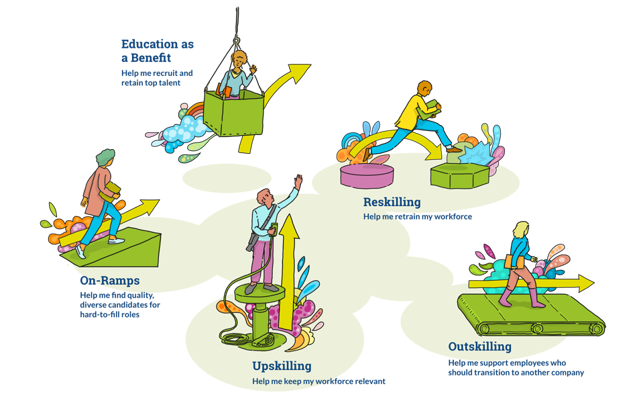
\includegraphics[width=0.6\linewidth,keepaspectratio]{career1}
\end{center}

{\tiny (Ref: As Pressure To Upskill Grows, 5 Models Emerge – Forbs.com)}
\end{frame}


%%%%%%%%%%%%%%%%%%%%%%%%%%%%%%%%%%%%%%%%%%%%%%%%%%%%%%%%%%%
\begin{frame}[fragile]\frametitle{McKinsey Global Institute Report – Discussion Paper 2018}



\begin{center}
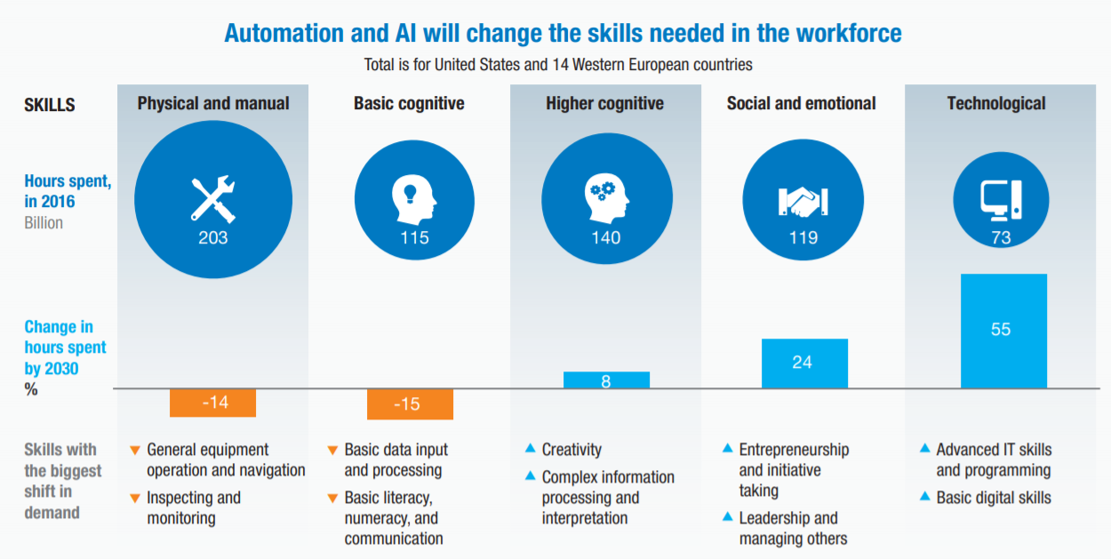
\includegraphics[width=\linewidth,keepaspectratio]{career2}
\end{center}

\end{frame}



%%%%%%%%%%%%%%%%%%%%%%%%%%%%%%%%%%%%%%%%%%%%%%%%%%%%%%%%%%%
\begin{frame}[fragile]\frametitle{Examples}
\begin{columns}
    \begin{column}[T]{0.5\linewidth}
		Less mechanical, automatable

      \begin{itemize}
		\item Bill and account collectors
		\item Data entry operators
		\item Computer network support 
		\item Secretaries and administrative assistants
		\item Insurance sales agents
		\item Office clerks

	  \end{itemize}
\begin{center}
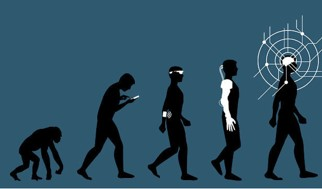
\includegraphics[width=\linewidth,keepaspectratio]{career3}
\end{center}

{\tiny (Source: The Simplistic Debate Over Artificial Intelligence – Preston Estep
)}

    \end{column}
    \begin{column}[T]{0.5\linewidth}
		More Cognitive, Creative, Human

      \begin{itemize}
		\item Software developers
		\item Customer service representatives
		\item General and operations managers
		\item Human resources managers
		\item Personal finance advisors
		\item Psychologists
		\item Artists
		\item Sportsman
		\item Researchers
		\item Nurses, care

	  \end{itemize}
    \end{column}
  \end{columns}
\end{frame}



% %%%%%%%%%%%%%%%%%%%%%%%%%%%%%%%%%%%%%%%%%%%%%%%%%%%%%%%%%%%
% \begin{frame}[fragile]\frametitle{Sample List Slide}

% \begin{itemize}
% \item aaa
% \end{itemize}
	  
% \end{frame}

% %%%%%%%%%%%%%%%%%%%%%%%%%%%%%%%%%%%%%%%%%%%%%%%%%%%%%%%%%%%
% \begin{frame}[fragile]\frametitle{Sample Picture Inclusion}

% \begin{center}
% \includegraphics[width=0.8\linewidth,keepaspectratio]{myphoto}
% \end{center}	  
% \end{frame}

% %%%%%%%%%%%%%%%%%%%%%%%%%%%%%%%%%%%%%%%%%%%%%%%%%%%
% \begin{frame}[fragile] \frametitle{Sample Code Listing}
% \begin{lstlisting}
% import aaa
% \end{lstlisting}

% \end{frame}

% %%%%%%%%%%%%%%%%%%%%%%%%%%%%%%%%%%%%%%%%%%%%%%%%%%%%%%%%%%%
% \begin{frame}[fragile]\frametitle{Sample Two Columns Slide}
% \begin{columns}
    % \begin{column}[T]{0.6\linewidth}
      % \begin{itemize}
		% \item aaa
	  % \end{itemize}

    % \end{column}
    % \begin{column}[T]{0.4\linewidth}
      % \begin{itemize}
		% \item bbb
	  % \end{itemize}
    % \end{column}
  % \end{columns}
% \end{frame}

% %%%%%%%%%%%%%%%%%%%%%%%%%%%%%%%%%%%%%%%%%%%%%%%%%%%%%%%%%%%%%%%%%%%%%%%%%%%%%%%%%%%
% \begin{frame}[fragile]\frametitle{Sample Tabular Data}

% aaa

% \begin{tabular}{|c|c|}
	% \hline
	% Platform & Time (s) \\
	% \hline \hline
	% Python & $\sim$1500.0 \\
	% \hline
	% NumPy & 29.3 \\
	% \hline
	% Matlab & $\sim$29.0 \\
	% \hline
	% Octave & $\sim$60.0 \\
	% \hline
	% Blitz (C++) & 9.5 \\
	% \hline
	% Fortran & 2.5 \\
	% \hline
	% C & 2.2 \\
	% \hline
% \end{tabular}

% \end{frame}
